%%%%%%%%%%%%%%%%%%%%%%%%%%%%%%%%%%%%%%%%%
% University Assignment Title Page 
% LaTeX Template
% Version 1.0 (27/12/12)
%
% This template has been downloaded from:
% http://www.LaTeXTemplates.com
%
% Original author:
% WikiBooks (http://en.wikibooks.org/wiki/LaTeX/Title_Creation)
%
% License:
% CC BY-NC-SA 3.0 (http://creativecommons.org/licenses/by-nc-sa/3.0/)
% 
% Instructions for using this template:
% This title page is capable of being compiled as is. This is not useful for 
% including it in another document. To do this, you have two options: 
%
% 1) Copy/paste everything between \begin{document} and \end{document} 
% starting at \begin{titlepage} and paste this into another LaTeX file where you 
% want your title page.
% OR
% 2) Remove everything outside the \begin{titlepage} and \end{titlepage} and 
% move this file to the same directory as the LaTeX file you wish to add it to. 
% Then add \input{./title_page_1.tex} to your LaTeX file where you want your
% title page.
%
%%%%%%%%%%%%%%%%%%%%%%%%%%%%%%%%%%%%%%%%%
%\title{Title page with logo}
%----------------------------------------------------------------------------------------
%	PACKAGES AND OTHER DOCUMENT CONFIGURATIONS
%----------------------------------------------------------------------------------------

\documentclass[12pt]{article}
\usepackage[english]{babel}
\usepackage[utf8x]{inputenc}
\usepackage{amsmath}
\usepackage[colorinlistoftodos]{todonotes}
\usepackage[font={footnotesize,it}]{caption}
\usepackage{multicol}
\usepackage{graphicx}
\usepackage[colorinlistoftodos]{todonotes}
\usepackage[center]{caption}
\newenvironment{Figure}
 {\par\medskip\noindent\minipage{\linewidth}}
{\endminipage\par\medskip}
\graphicspath{{text-mining/figs/}}
\usepackage{subcaption}
\usepackage[
backend=biber,
style=numeric,
sorting=ynt,
]{biblatex}

\addbibresource{references.bib}
\begin{document}

\begin{titlepage}

\newcommand{\HRule}{\rule{\linewidth}{0.5mm}} % Defines a new command for the horizontal lines, change thickness here

\center % Center everything on the page
 
%----------------------------------------------------------------------------------------
%	HEADING SECTIONS
%----------------------------------------------------------------------------------------

\textsc{\LARGE Università degli studi di Milano-Bicocca}\\[1cm] % Name of your university/college
\textsc{\Large Text Mining And Search}\\[0.3cm] % Major heading such as course name
\textsc{\large Final Project}\\[0.1cm] % Minor heading such as course title

%----------------------------------------------------------------------------------------
%	TITLE SECTION
%----------------------------------------------------------------------------------------

\HRule \\[0.4cm]
{ \huge \bfseries Sentiment Analysis of Amazon Reviews}\\[0.4cm] % Title of your document
\HRule \\[1.5cm]
 
%----------------------------------------------------------------------------------------
%	AUTHOR SECTION
%----------------------------------------------------------------------------------------

\large
\emph{Authors:}\\
Lorenzo Camaione - 850380 - l.camaione@campus.unimib.it \\   % Your name
Davide Toniolo - 800458- d.toniolo2@campus.unimib.it   \\[1cm] % Your name

% If you don't want a supervisor, uncomment the two lines below and remove the section above
%\Large \emph{Author:}\\
%John \textsc{Smith}\\[3cm] % Your name

%----------------------------------------------------------------------------------------
%	DATE SECTION
%----------------------------------------------------------------------------------------

{\large \today}\\[1cm] % Date, change the \today to a set date if you want to be precise

%----------------------------------------------------------------------------------------
%	LOGO SECTION
%----------------------------------------------------------------------------------------
\begin{center}
\begin{Figure}
\centering{

\includegraphics{figs/logo.png}\\[1cm] % Include a department/university logo - this will require the graphicx package
}
\end{Figure}
\end{center}
 
%----------------------------------------------------------------------------------------

\vfill % Fill the rest of the page with whitespace

\end{titlepage}


\begin{abstract}
In this paper a number of solution for a text classification task are presented. The objective of the project is to predict, from its text, whether the rating of a review is either positive or negative. The dataset consists of reviews of fashion products sold on Amazon. The different models evaluated perform well, but their results are skewed towards the most frequent class. 
\end{abstract}

\section{Introduction}
Sentiment analysis consists of classifying a document in a set of predefined categories. In its simplest form, the emotions are positive or negative, while more complex analyses use a greater number of classes.

The dataset used in this project is a collection of Amazon reviews regarding some specific classes of products. In particular the products chosen are either clothes, shoes or jewellery. This dataset is made available directly by Amazon. The data span a period of 18 years, including a large number of reviews up to March 2013. The objective of the project is to develop a model capable of predicting the rating of a review from its textual content.

In the Amazon e-commerce people usually review products they buy. In this process they typically choose a rating between 1 and 5 and then add a text to try to explain why they picked that rating.

The reviews having either one star and five stars have been explored creating a word cloud for each group. These word clouds don't contain stop-words.
\begin{figure}[h]
    \center
    \begin{subfigure}{0.49\textwidth}
    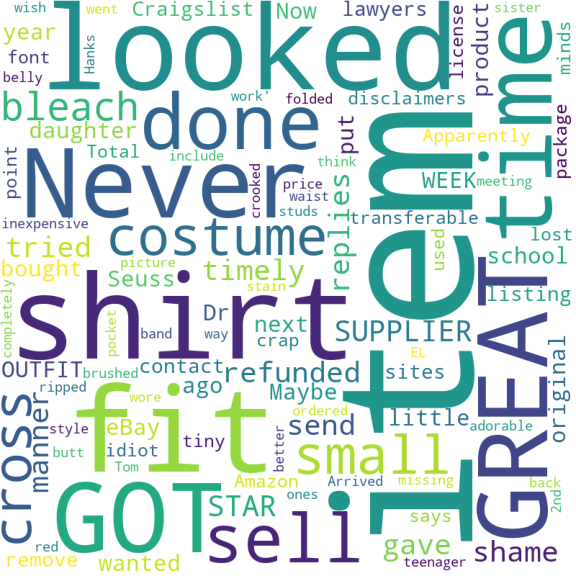
\includegraphics[width=0.9\linewidth, height=5cm]{onestar_wordcloud.png}
    \caption{One star reviews wordcloud}
    \label{5*cloud}
    \end{subfigure}
    \begin{subfigure}{0.49\textwidth}
    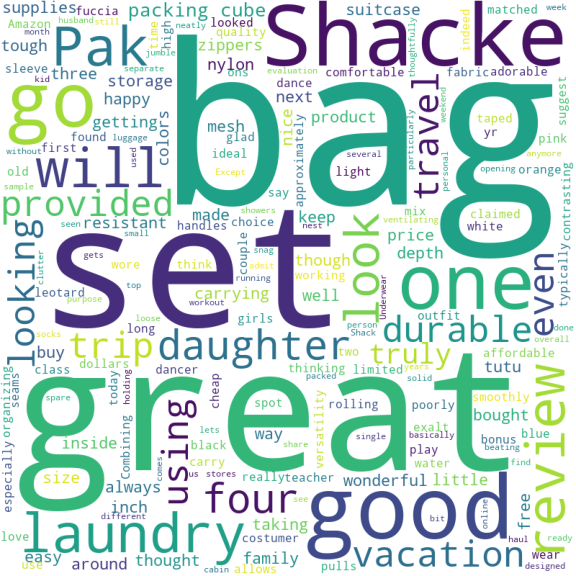
\includegraphics[width=0.9\linewidth, height=5cm]{fivestar_wordcloud.png}
    \caption{Five star reviews wordcloud}
    \label{1*cloud}
    \end{subfigure}
\end{figure}

Looking at the word clouds it's clear that there are some differences. Although some words are in both word clouds, others are not: the one star word cloud has words like \textit{never} and \textit{crap} while the five stars one has words like \textit{great} and \textit{good}. The two word clouds look different, but the majority of the words are shared between the two.

\section{The Dataset}
The dataset consists of 280 000 reviews collected from the \textit{Clothing, Shoes and Jewellery} products of the Amazon online store in the May 1996 - July 2014 time frame \cite{HeAuley}, \cite{Auley}. It comes as a sequence of JSON documents with the following attributes:
\begin{itemize}
    \item \texttt{reviewerID} - ID of the reviewer
    \item \texttt{asin} - ID of the product
    \item \texttt{reviewerName} - name of the reviewer
    \item \texttt{helpful} - helpfulness rating of the review. It is a array of ints and of length 2. A value of \texttt{[1, 2]} means that among the two users that viewed that review, one of them found it useful.
    \item \texttt{reviewText} - the text of the review
    \item \texttt{overall} - rating of the product. Floating point number, 1 to 5. There are no fractional ratings.
    \item \texttt{summary} - the summary of the review made by the author
    \item \texttt{unixReviewTime} - the time when the review was posted in an human-readable (American) format.

The overall file size is 150 MB.
\end{itemize}
The target variable class frequencies are showed in the following histograms: in the first one it is shown as is in the dataset while in the second one the histogram shows the variable after it has been discretized.
\begin{figure}[h]
    \center
    \begin{subfigure}{0.49\textwidth}
    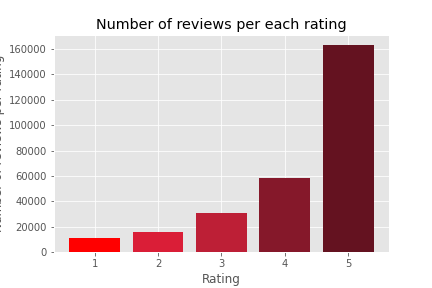
\includegraphics[width=0.9\linewidth, height=5cm]{frequencies_classes.png}
    \caption{Frequencies of the target variable overall}
    \label{5*cloud}
    \end{subfigure}
    \begin{subfigure}{0.49\textwidth}
    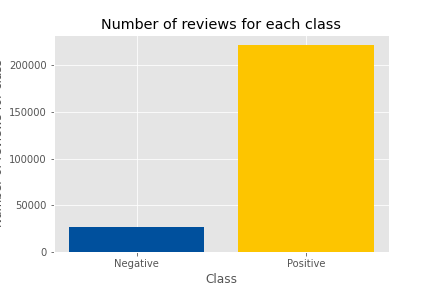
\includegraphics[width=0.9\linewidth, height=5cm]{frequencies_neg_pos.png}
    \caption{Frequencies of the target variable after it has been discretized}
    \label{1*cloud}
    \end{subfigure}
\end{figure}

\section{The Methodological Approach}
Different NLP pipelines and different classifiers are compared in terms of results and speed.

\subsection{Preprocessing}
As soon as the file is read, the relevant fields are extracted and everything else gets discarded. Given that the task consists of classifing the review into positive or negative given the textual content, only the fields \texttt{reviewText} (input variable) and \texttt{overall} (target variable) are kept. The latter is then transformed so that the 1 and 2 classes are encoded as 0 (negative) and the 4-5 starts as 1 (positive). The neutral 3 star reviews are discarded.

\subsection{Tokenization}
The raw textual data isn't suitable for manipulation by a machine, so it needs to be transformed into a more computer-friendly form. This transformation consists of a series of operations, the first of which is called \textit{tokenization}.
A \textit{token} is a single, self contained "piece of text". Splitting each sentence into words isn't sufficient: a concept or idea may be represented by multiple words and if this is the case, separating them may lead to worse results.


As an example, the sentence "John wants to visit Italy this summer" can be naïvely tokenized by splitting into words, but in the sentence "Catherine has found a new state of the art model for NLP!" the words "state of the art" represent a single concept and shouldn't be separeted.

A great variety of algorihtms for tokenization are available. For this project the method \texttt{word\_tokenize} by \texttt{nltk} was used.

\subsection{Stop Words Removal}
When building a vocabulary, it is often the case that the most frequent words (or tokens) are not the most informative. For example, in the English language "the" is by far the most common word, but it is hardly of any use to discern documents. A common practice is to remove words that occur too frequently, in order to reduce the size of the vocabulary and reduce the number of features.

\texttt{nltk}'s stop-words list for the english language was used.

\subsection{Stemming and Lemmatization}
These terms refer to two related practices used to reduce vocabulary size and improve computability: a given word is reduced to its root (e.g. "giver" becomes "give").
Stemming is a more crude and less sophisticated approach, but a more faster one.


\subsection{Choosing the Text Representation}
The preprocessed text then needs to be encoded in some form that is suitable to the classification algorithms that the researcher wishes to use.

The simplest of all use "unigrams" (that are, single tokens): they make use of each token in the document individually, without regard for their order or semantic/logical relationship with each other. The output of these encoding approaches is a matrix $W$ in which the first axis refers to the vocabulary entries, while the second refers to the document in the corpus.

The entries of $W$ can be obtained in different ways and each approach gets its own unique name:
\begin{itemize}
    \item set of words - $W_{ij}$ is a boolean that records the presence or absence of the $i$-th token in the $j$-th document.
    \item bag of words - $W_{ij}$ is the number of times the $i$-th token appears in the $j$-th word.
    \item various weighting schemes: document length, max tf, tf-idf.
\end{itemize}

For this project the set of words and the tf-idf approaches where used. Bi-grams tecniques and higher have not been explored, given that they have much higher memory requirements (approx quadratic and cubic respectively).

\subsection{Reducing Memory Usage}
Even with a simple unigram text representation, if the document corpus is large enough, the $W$ matrix can occupy a significant portion of memory, several GB in size.

To address this problem, tokens that are either too common or too rare can be excluded. Then, the matrix can be decomposed using PCA or some other dimentionality reduction technique.

To compute the matrix \texttt{sklearn}'s \texttt{Tf-idf} class was used. The advantages of Scikit-Learn's implementation are twofold: firstly, their code is fast, faster than a simple Python implementation by the end user would likely be. Second, they output a sparse matrix. Given that many of the entries of the $W$ are usually 0, this hack allows for a huge memory saving. Also, when used for fitting compatible (both algorithm-wise and implementation-wise) classifiers, this can greatly reduce the number of computations required.

The dimensionality of the matrix is reduced using Trucated SVD (i.e. PCA where only the components corresponding to the higher variances are retained). By doing so, a dense matrix of much lower dimension is obtained: the number of output features is set to 100, the default.

\subsection{Classification}
Different Machine Learning classification algorithms were explored and evaluated. Given that the dataset is highly unbalanced, the performances of the different classifiers were compared using the precision and recall metrics.

In order to obtain a balanced fit out of the unbalanced dataset, each class was weighted with the moltiplicative inverse of its relative frequency: in principle a weighting scheme like this allows the researcher to use all the available training data and still get a classifier that doesn't favor the most frequent classes.

This technique was used with all the algorithms, with the sole exception of the K Nearest Neighbours classifier, given that it doesn't make sense in this case.

% Please add the following required packages to your document preamble:
% \usepackage{graphicx}
\section{Results and Evaluation}
\begin{table}[]
\begin{tabular}{|l|l|l|l|l|l|l|}
\hline
&
  Metric &
  Gaussian NB &
  Random Forest &
  kNN &
  Linear SVM &
  ANN \\
  \hline
  & Precision & 0.18 & 0.75 & 0.24 & 0.32 & 0.37 \\
  Class 0 & Recall & 0.74 & 0.10 & 0.34 & 0.84 & 0.82 \\
  & F1-measure & 0.28 & 0.18 & 0.28 & 0.46 & 0.51 \\
  \hline
  & Precision & 0.95 & 0.90 & 0.84 & 0.98 & 0.97 \\
  Class 1 & Recall & 0.58 & 1.00 & 0.87 & 0.79 & 0.83 \\
  & F1-measure & 0.72 & 0.95 & 0.86 & 0.87 & 0.90 \\
  \hline
  & Precision & 0.56 & 0.82 & 0.43 & 0.65 & 0.67 \\
  Macro Avg & Recall & 0.66 & 0.55 & 0.43 & 0.81 & 0.83 \\
  & F1-measure & 0.50 & 0.56 & 0.42 & 0.67 & 0.70 \\
  \hline
  Accuracy & & 60\% & 90\% & 73\% & 79\% & 83\& \\
  \hline
\end{tabular}
\caption{The performances of the various classificators. Results on the positive class are better across the board.}
\label{tab:class}
\end{table}



Obtaining high levels of the target metrics was a challenging task. As showed in table \ref{tab:class}, even with the weighting of the classes during the training stage, the classifiers still perform better on the positive reviews across the board.

Perhaps the problem could be solved by a more aggressive weighting scheme. However, various trials showed disappointing results.

This, coupled with the fact that the unbalanced results are common to all the classifiers, leads to the intuition that the problem may be lying in the data. The word clouds for the negative and positive reviews \ref{5*cloud} and \ref{1*cloud}, are very similar. Maybe, even with the tf-idf scheme (that should penalize words that are common across all documents).

Thus, the problem may lie in the use of a unigram representation.

Another issue may be the dimentionality reduction technique used: the truncated SVD selects the components associated with the highest variance. However, this variance could be common to all the classes and thus of limited use when classifying.

For example, the highest variance components could be associated with the different subcategories of the dataset (e.g. clothing vs shoes vs jewelley) and would be useful for topic detection, but not for sentiment analysis.

Therefore, a filter that is capable of retaining the features that have the highest variance \textit{between} the classes might be able to improve the results.


\section{Conclusions and Future Work}
The NLP piepeline and classifiers used show sufficiently high metrics. The text preprocessing is able to extract the features from the text without using an excessive amount of memory.

However, the unbalanced results obtained by the classifiers suggests that a more sophisticated text representation method might improve the final scores.

Also, using a dimentionality reduction technique that is able to keep the most informative features will likely help.

\printbibliography
\end{document}